% The San Francisco Social Media Data and Analytics Group
% 05 November 2013
% Scott Hendrickson
% @DrSkippy27
% Gnip

\documentclass{beamer}
\setbeamertemplate{navigation symbols}{}

% THEMES
\usetheme{gnip}
% PACKAGES
\usepackage[group-separator={,}]{siunitx}
%\usepackage{fontspec}
\usepackage{graphicx}
% FOOTER
\setbeamertemplate{footline}[text line]{
\colorbox{white}{\parbox[22px]{\paperwidth} {\color{linecolour} {\line(1,0){500} \\ \hfill @DrSkippy27 @gnip}}}
}
\beamersetuncovermixins{\opaqueness<1>{25}}{\opaqueness<2->{15}}

\usepackage{minted}
\usepackage{tikz}

\begin{document}

\title{Data Scientist's Approach to Social Data}
\author{Scott Hendrickson \\ Principal Data Scientist, Gnip \\  @DrSkippy27}
\date{\today} 

% title

\begin{frame}
\titlepage
\end{frame}

%%%%%%%%
\section{Social Data}
{
\usebackgroundtemplate{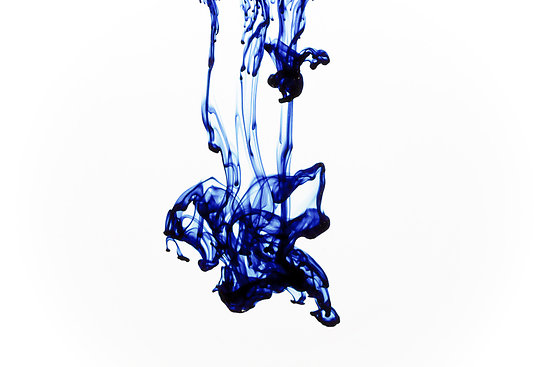
\includegraphics[width=4cm]{./imgs/ink.jpg}}
\begin{frame}
\textcolor{black} {
\hfill \Huge \insertsection}
\end{frame}
}

\begin{frame}\frametitle{Social data}
\begin{center}
{\Huge created by \\ [8pt] interactions \\ [15pt] among people}
\end{center}
\end{frame}

\begin{frame}\frametitle{Social data}
\begin{center}
{\Huge form and content \\ [8pt] shaped by \\ [15pt] people's behavior}
\end{center}
\end{frame}

\begin{frame}\frametitle{Sources}
{\Huge
\begin{itemize}
\item firehoses
\item APIs
\item scraping
\end{itemize}
}
\end{frame}

% Firehoses

\begin{frame}\frametitle{Firehose}
\begin{center}
{\Huge Continuous stream \\ [8pt] of activities \\ [15pt] in near-real time}
\end{center}
\end{frame}

% Activity 

\begin{frame}\frametitle{Activity}
\begin{center}
{\Huge people interacting \\ [8pt] on social media platform}
\end{center}
\end{frame}

% Volumes

\begin{frame} \frametitle{Firehose volumes}
\begin{table}
\begin{tabular}{l|r}
\hline
   {Publisher}   &   {Daily Activity}   \\
\hline 
    Twitter      &      500M   \\
    Tumblr      &       105M   \\
    Foursquare &       4.3M \\
    GetGlue &         430k \\
    Wordpress Posts &     919k   \\
    Wordpress Comments & 1.7M \\
    Disqus       &       1.9M  \\
    Engagement (likes, votes) & 59M  \\
\hline
\end{tabular}
\end{table}
\end{frame}

%
\begin{frame}\frametitle{Every day @Gnip}
\begin{center}
{\Huge $\frac{3}{4}$ Billion IN \\ [18pt] 4 Billion OUT}
\end{center}
\end{frame}

%%%%%%%%
\section{Analysis}
{
\usebackgroundtemplate{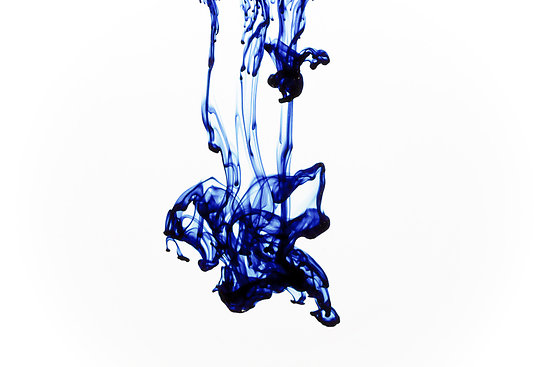
\includegraphics[width=4.5cm]{./imgs/ink.jpg}}
\begin{frame}
\textcolor{black} {
\hfill \Huge \insertsection}
\end{frame}
}

% Feels like this
\begin{frame}
  \begin{center}
    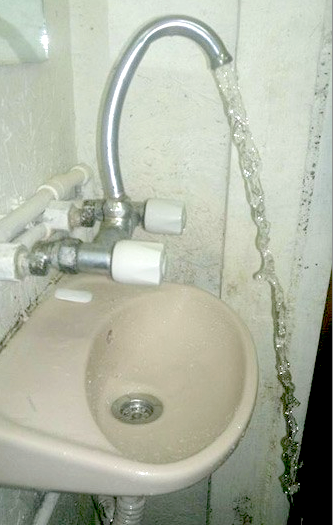
\includegraphics[height=9cm]{./imgs/sinkfail.png}
  \end{center}
\end{frame}


% Source considerations

\begin{frame}\frametitle{Analysis considerations}
{\Large
\begin{itemize}
\item Technology - interfaces, tools, infrastructure for accessing
\item Latency - how soon after activity as created?
\item Uniformity - how hard/costly to normalize data formats?
\item Coverage - do you need it all? a defined sample?
\item Meta-data -  how much and what kind of data about the data?
\end{itemize}
}
\end{frame}

% Source considerations

\begin{frame}\frametitle{Business considerations}
{\Large
\begin{itemize}
\item Licensing - do you have the right to analyze, display, store data?
\item Terms-of-Service Compliance - violating publishers terms of service, privacy protections?
\item Cost - data collection costs? licensing costs? processing and storage costs?
\item Analysis mode - batch vs. real-time? event vs. background? time, structure, language, people?
\end{itemize}
}
\end{frame}

% what are we doing?

% models drive analysis ; analysis drives model picture

\begin{frame}\frametitle{Models \ldots}
{\Large
\begin{itemize}
\item domains - events, time series, language analysis, graph structures, etc.
\item drives storage, analysis and access strategies, etc.
\item analysis objectives - detection, alerting, status dashboard, discovery projects, validation, etc.
\end{itemize}
}
\end{frame}

% Analysis choices
\begin{frame}\frametitle{Example analysis strategies}
  \begin{center}
    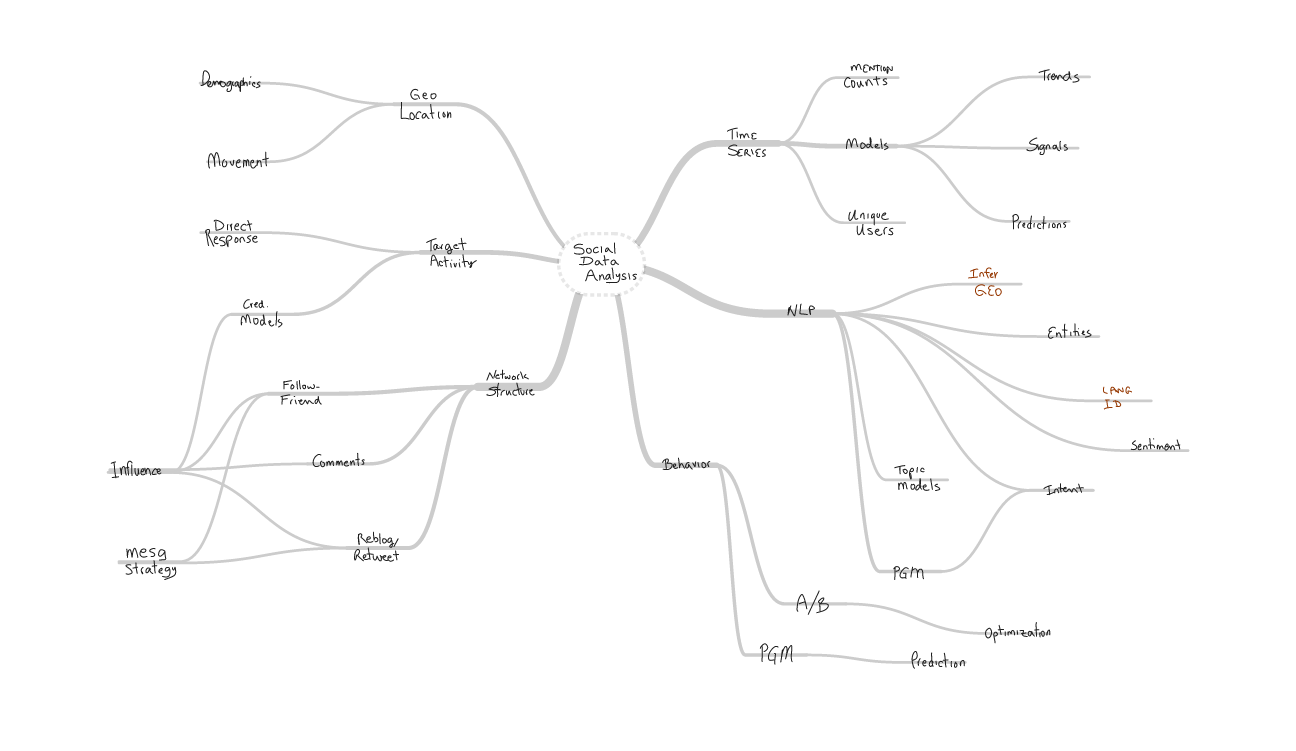
\includegraphics[width=11cm]{./imgs/mindmap.png}
  \end{center}
\end{frame}


% Reality is a little more ironic
\begin{frame}
  \begin{center}
    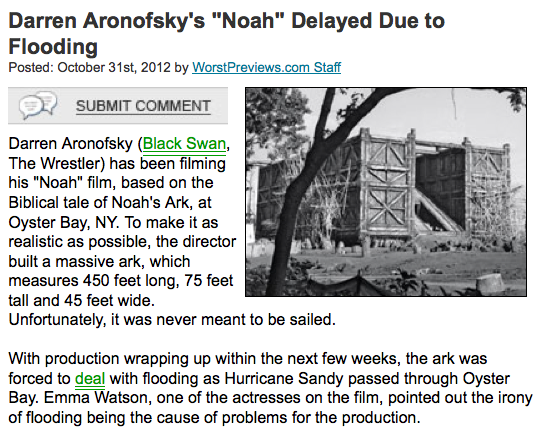
\includegraphics[height=11cm]{./imgs/flooding.png}
  \end{center}
\end{frame}

%%%%%%%%
%%
%%  EXAMPLES
%%
%%%%%%%%

%%%%%%%%
\section{Audience}
{
\usebackgroundtemplate{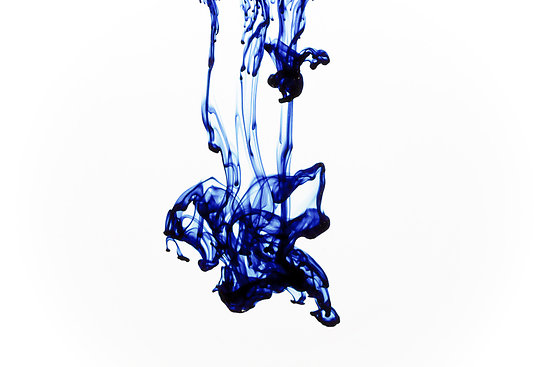
\includegraphics[width=5cm]{./imgs/ink.jpg}}
\begin{frame}
\textcolor{black} {
\hfill \Huge \insertsection}
\end{frame}
}

% toyota
\begin{frame}
  \begin{center}
    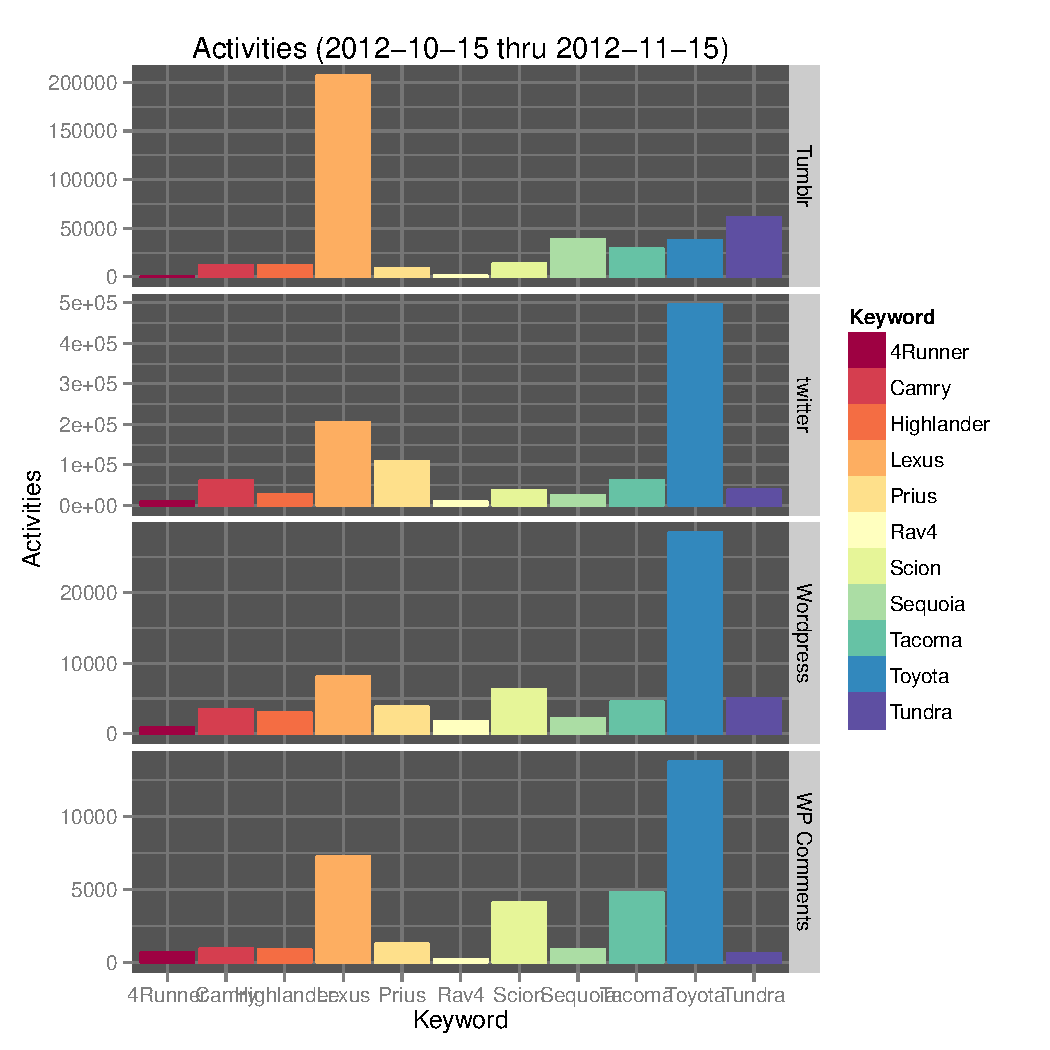
\includegraphics[width=8cm]{./imgs/TOY_bars.pdf}
  \end{center}
\end{frame}

% thanksgiving day
\begin{frame}
  \begin{center}
    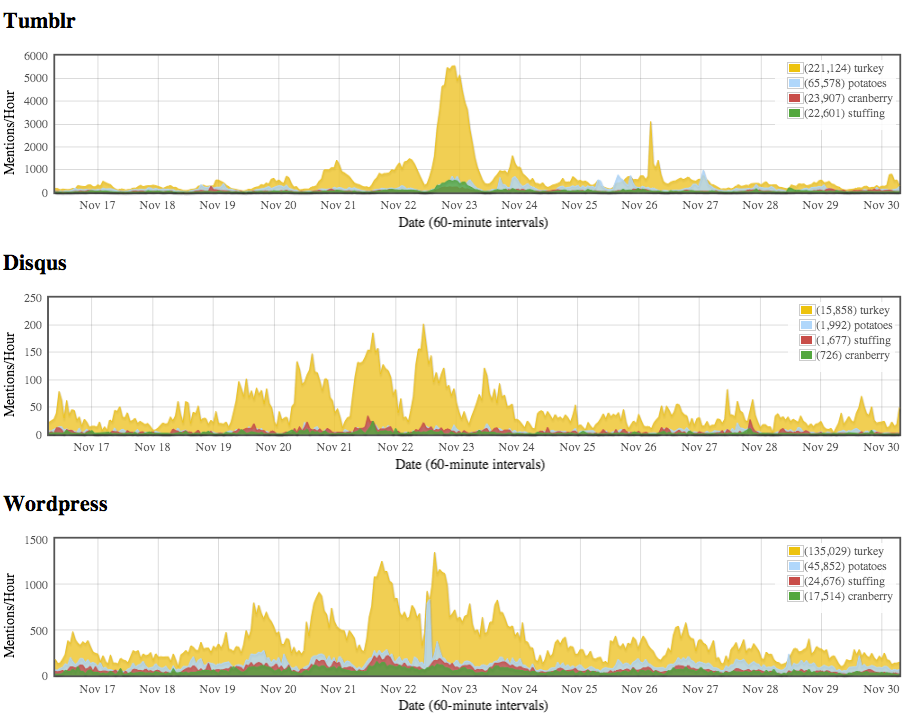
\includegraphics[width=10cm]{./imgs/t-day2012.png}
  \end{center}
\end{frame}

% thanksgiving day
\begin{frame}
  \begin{center}
    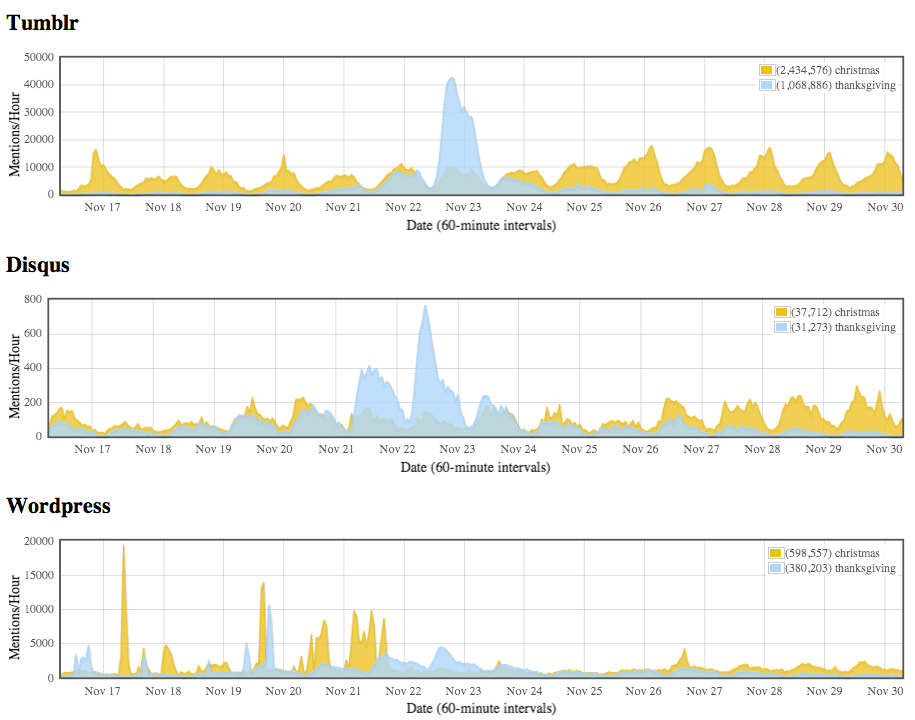
\includegraphics[width=10cm]{./imgs/t-dayvsx-mas.png}
  \end{center}
\end{frame}

% thanksgiving day
\begin{frame}
  \begin{center}
    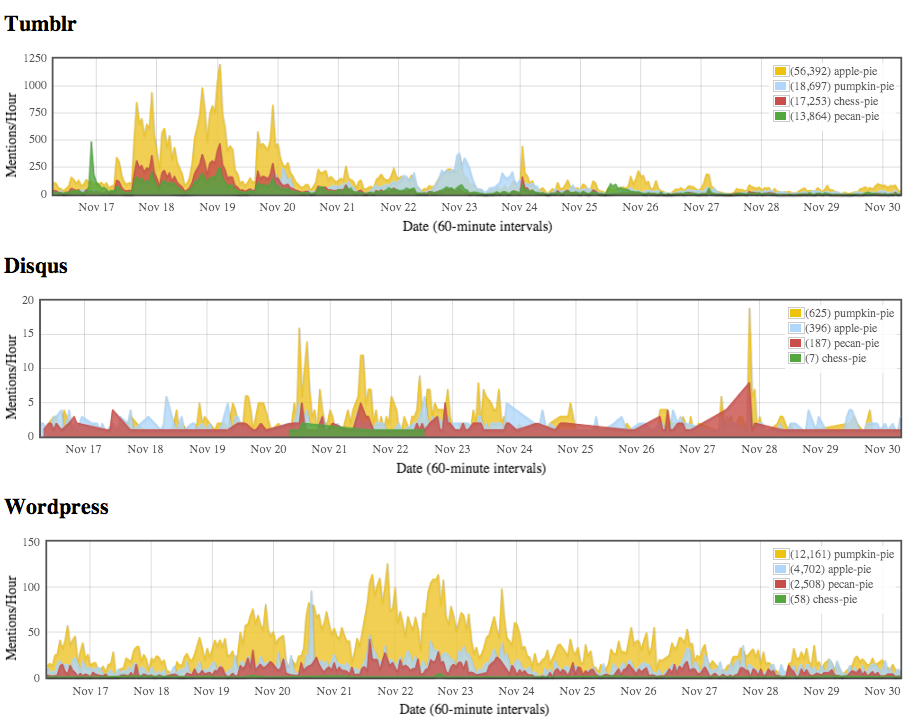
\includegraphics[width=10cm]{./imgs/pies2012.png}
  \end{center}
\end{frame}

%%%%%%%%
\section{Social Medial Pulse}
{
\usebackgroundtemplate{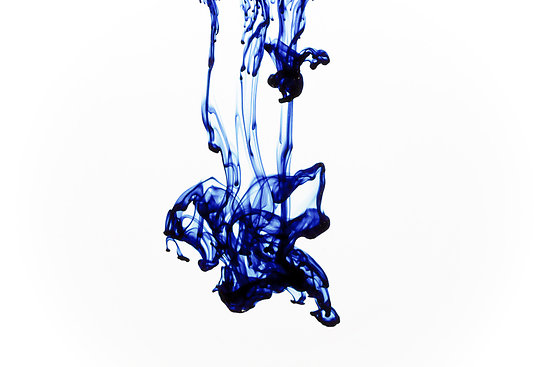
\includegraphics[width=5.5cm]{./imgs/ink.jpg}}
\begin{frame}
\textcolor{black} {
\hfill \Huge \insertsection}
\end{frame}
}

% social media pulse


% hurricane Irene

\begin{frame}\frametitle{Expected: hurricane}
  \begin{center}
    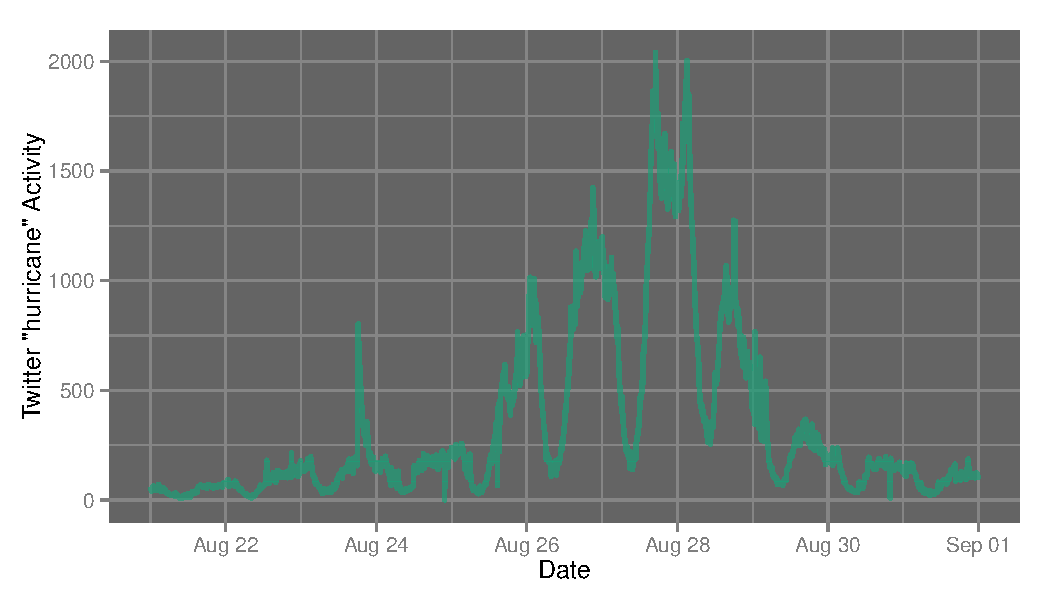
\includegraphics[width=11cm]{./imgs/SMP_hurricane.pdf}
  \end{center}
\end{frame}

\begin{frame}\frametitle{Unexpected: earthquake}
  \begin{center}
    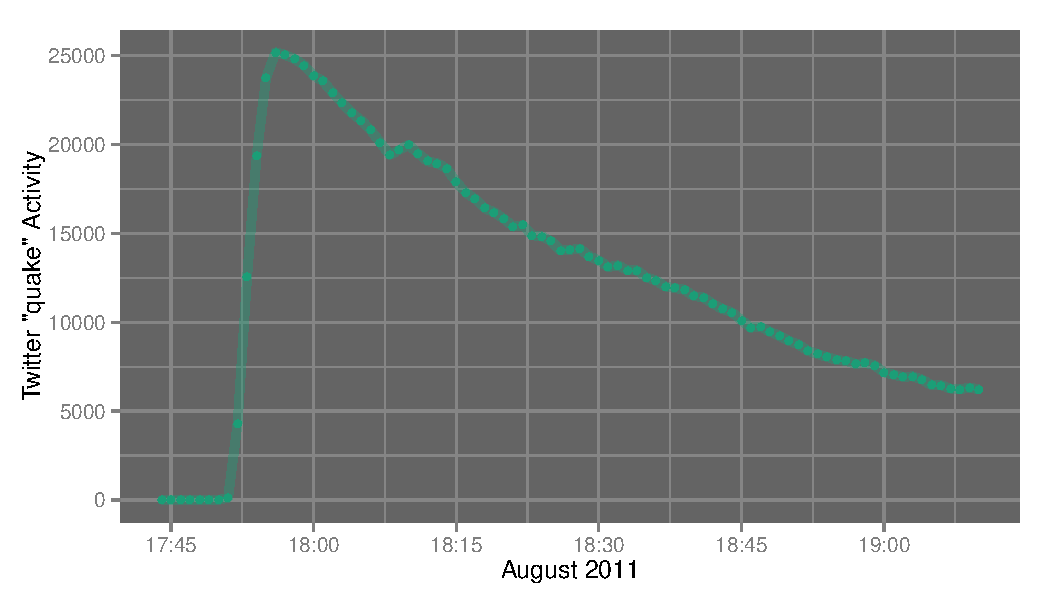
\includegraphics[width=11cm]{./imgs/SMP_va_quake.pdf}
  \end{center}
\end{frame}


% Events

\begin{frame}\frametitle{Classifying events}
\begin{table}
\begin{tabular}{ m{2cm} | m{ 2.5cm} | m{4cm}}
\hline
Type & Response & Examples \\ \hline
Expected    &  Build-up/Decay & Hurricane Sandy \newline Olympics \\ \hline
Unexpected (many obs.) & Social Media \newline Pulse & Beyonc\'{e} VMAs \newline  Mexico earthquake \newline  Steve Jobs \\ \hline
Unexpected  (network spread) & Network \newline Models  & Osama bin Laden \newline  Whitney Houston \newline  Syrian dissidents \\ \hline
\end{tabular}
\end{table}
\end{frame}


\begin{frame}\frametitle{Expected: hurricane}
  \begin{center}
    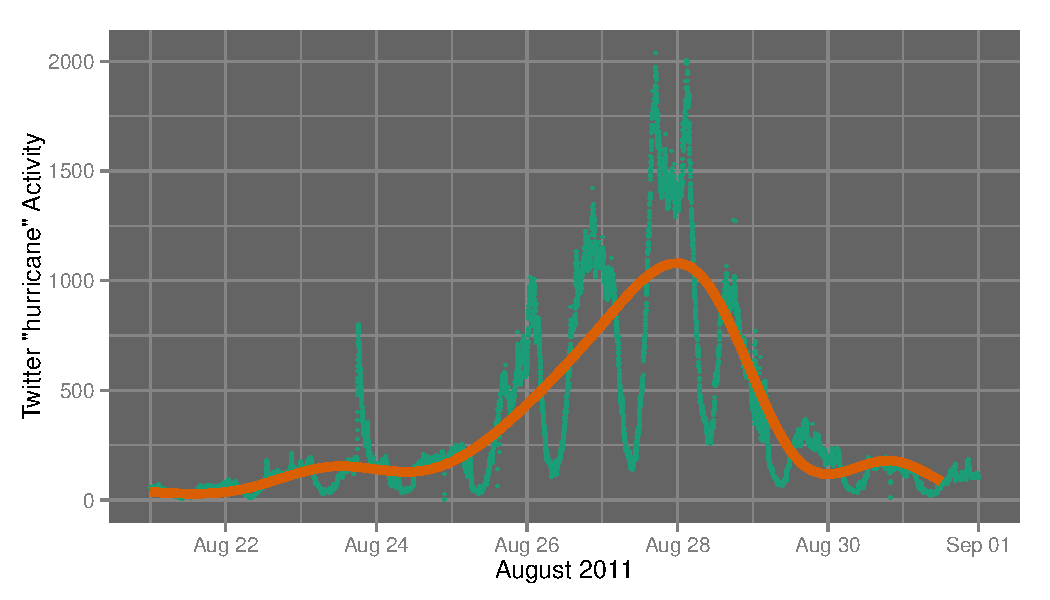
\includegraphics[width=11cm]{./imgs/SMP_hurricane_trend.pdf}
  \end{center}
\end{frame}


% half life

\begin{frame}\frametitle{Unexpected: earthquake}
  \begin{center}
    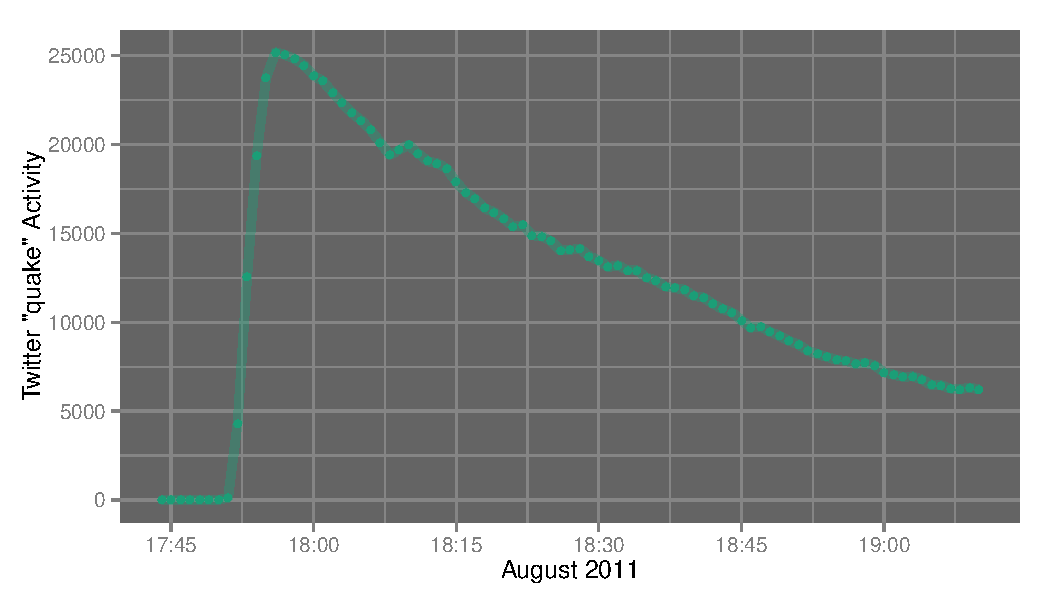
\includegraphics[width=11cm]{./imgs/SMP_va_quake.pdf}
  \end{center}
\end{frame}

\begin{frame}\frametitle{Half-life}
\begin{center}
{\Huge time to observe \\[6pt] $\frac{1}{2}$ of the activities \\[6pt] for an event}
\end{center}
\end{frame}

\begin{frame}
\frametitle{Social media pulse} 
Given an event, the probability of an activity from one person,

\begin{equation*}
f(t) = \lambda \exp(-\lambda t), \text{ for } t \geq 0.
\end{equation*}

Many people posting on same cue; so sum of random variables 

\begin{equation*}
S = X_1 + X_2 + \ldots + X_{n \text{ posters}}
\end{equation*}

Gamma probability distribution function,

\begin{equation*}
f_S(t) = \frac{ \beta^{-\alpha} t^{\alpha-1} \exp( \frac{-t}{\beta}) } {\Gamma(\alpha)}
\end{equation*}

Cumulative distribution is the ``generalized regularized incomplete gamma function'',

\begin{equation*}
F_S(t) = Q(\alpha, 0, \frac{ t}{\beta})
\end{equation*}
\end{frame}

% gamma plots

\begin{frame}
  \begin{center}
   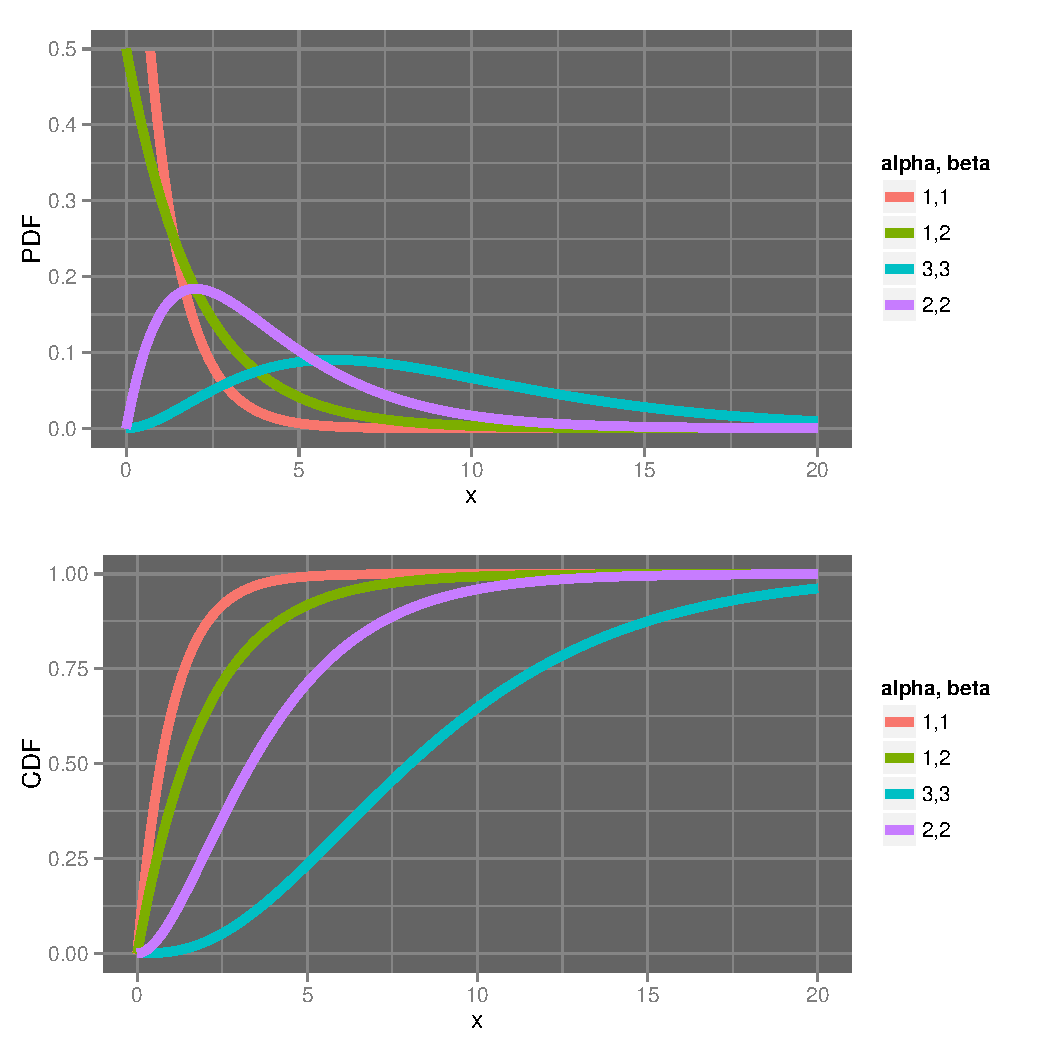
\includegraphics[height=6cm]{./imgs/SMP_gammadist.pdf}
  \end{center}
\end{frame}

\begin{frame}\frametitle{Why model half-life?}
{\Large
\begin{itemize}
\item predict total story volume
\item compare half-lives
\item anomalous story evolution
\end{itemize}
}
\end{frame}

\begin{frame}
  \begin{center}
    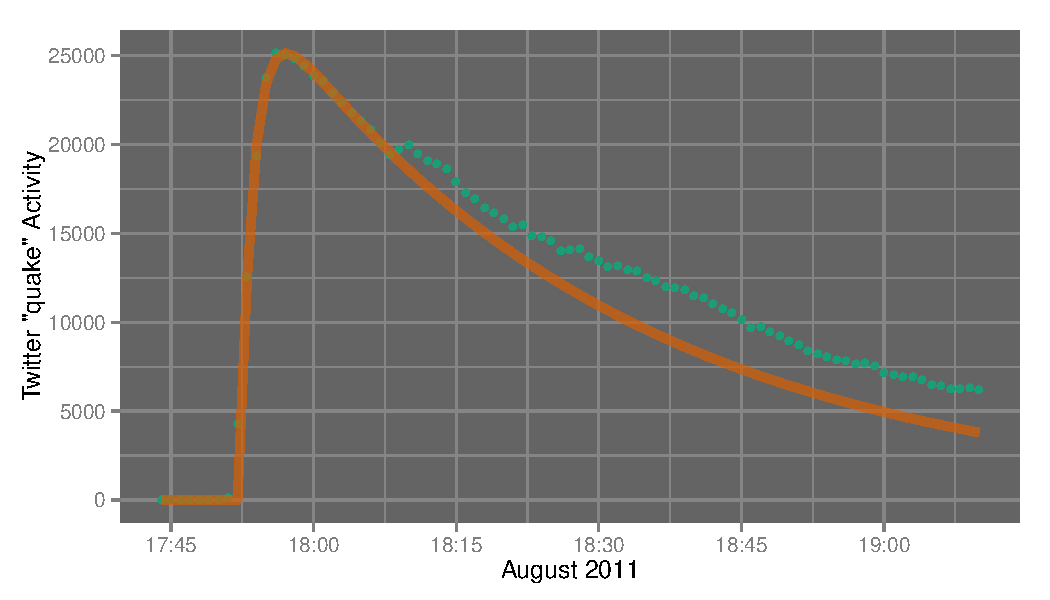
\includegraphics[width=8cm]{./imgs/SMP_va_quake_fit1.pdf}
  \end{center}
\end{frame}

% JPMorgan

\begin{frame}\frametitle{JPMorgan (-\$2B)}
 \hfill 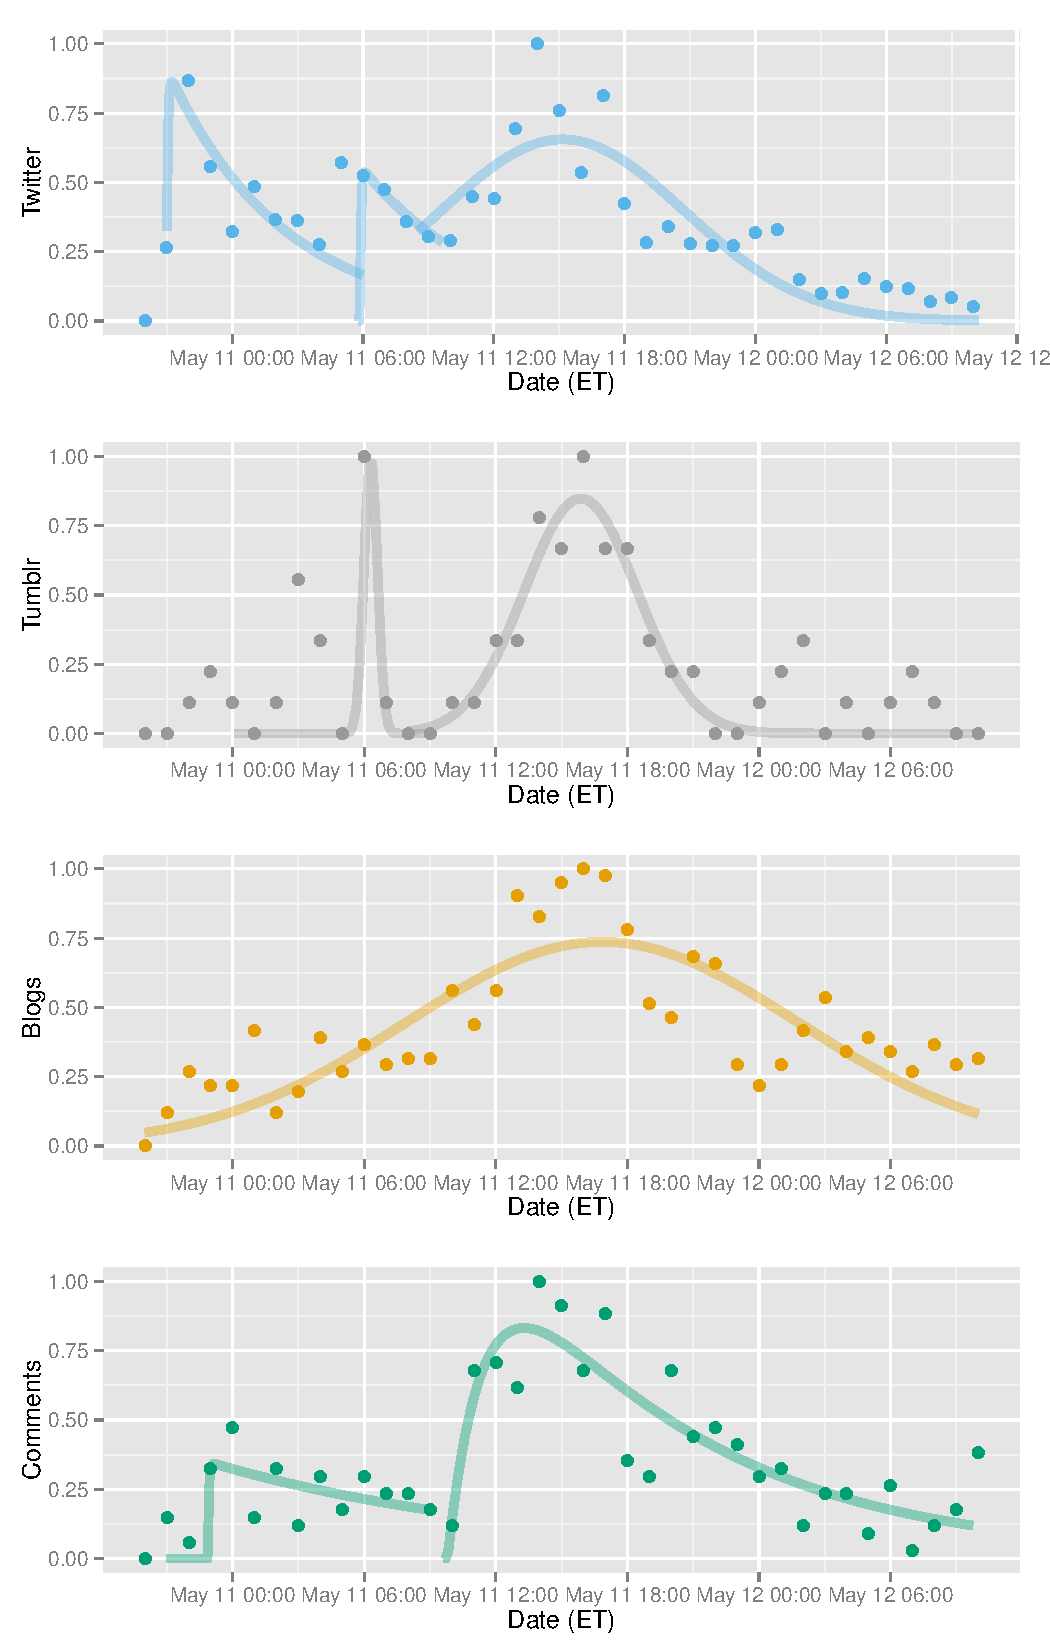
\includegraphics[height=8.0cm]{./imgs/SMP_JPMorgan.pdf}
\end{frame}


%%%%%%%%
\section{Structure}
{
\usebackgroundtemplate{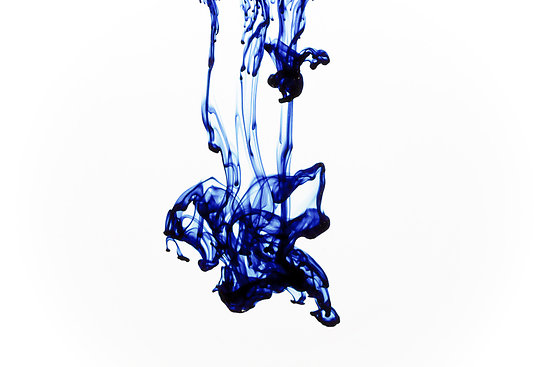
\includegraphics[width=6cm]{./imgs/ink.jpg}}
\begin{frame}
\textcolor{black} {
\hfill \Huge \insertsection}
\end{frame}
}

{
\usebackgroundtemplate{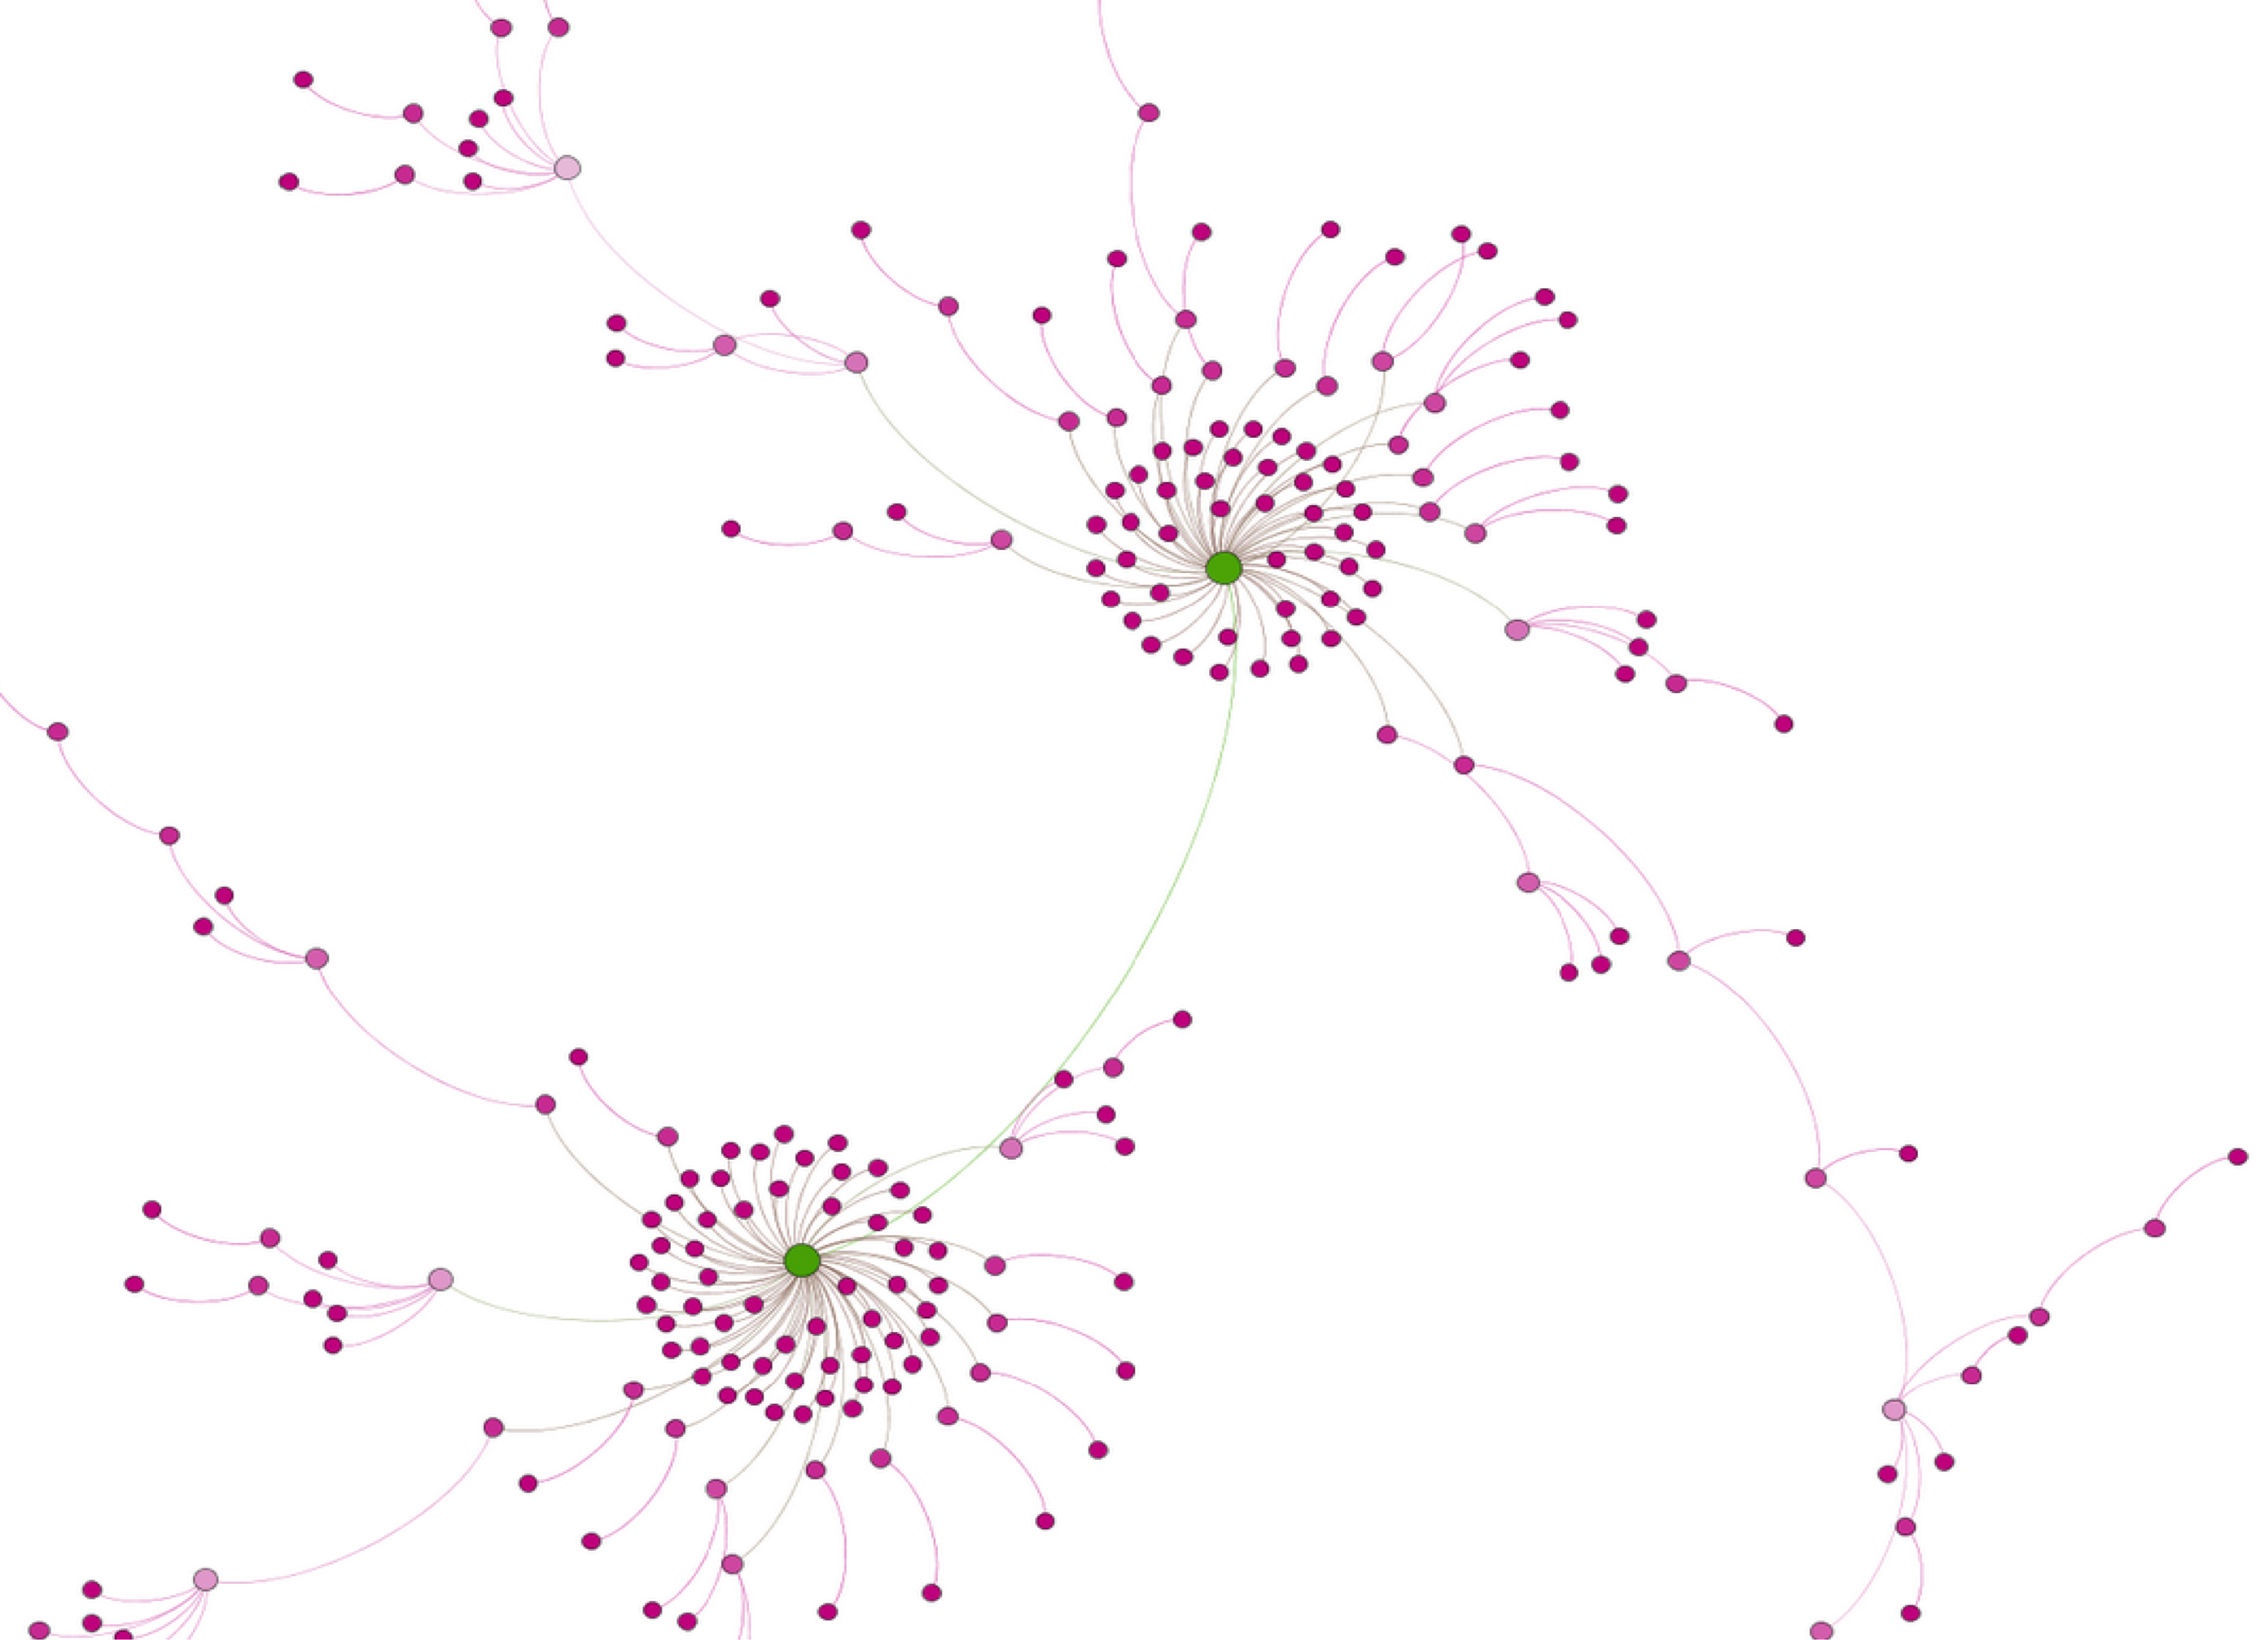
\includegraphics[width=\paperwidth]{./imgs/reblog_network.png}}
\begin{frame}
\textcolor{black} {
\vfill \hfill \Large Tumblr reblog network}
\end{frame}
}

{
\usebackgroundtemplate{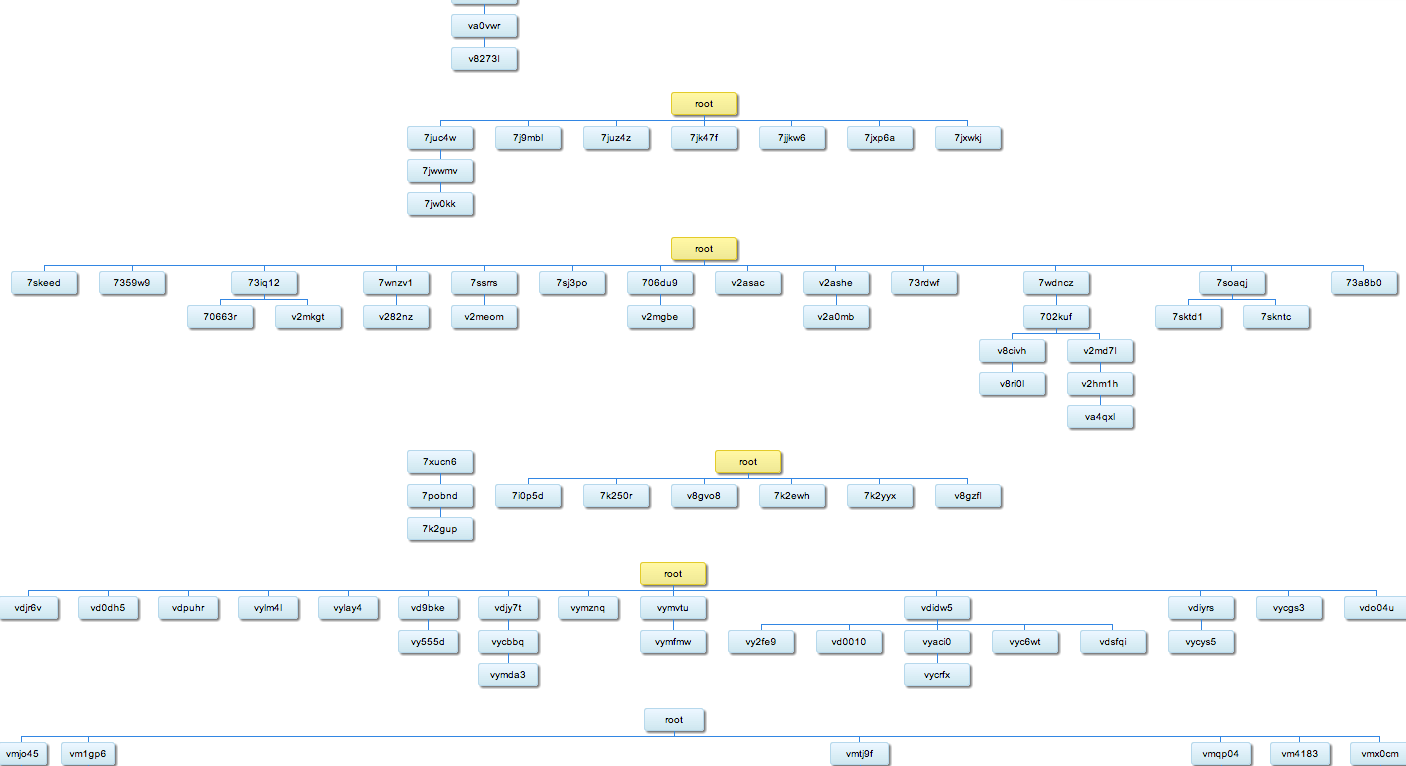
\includegraphics[width=\paperwidth]{./imgs/disqus_threads.png}}
\begin{frame}
\textcolor{black} {
\vfill \hfill \Large Disqus discussion threads}
\end{frame}
}

%%%%%%%%
\section{Structure and Language}
{
\usebackgroundtemplate{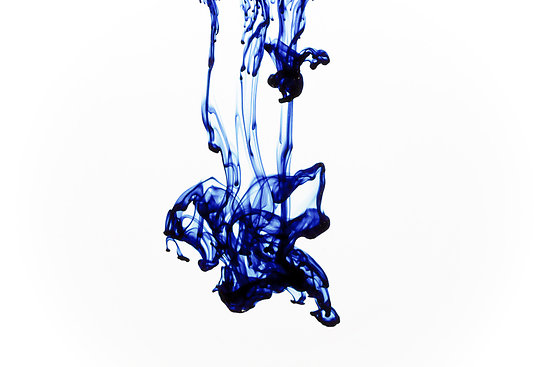
\includegraphics[width=6.5cm]{./imgs/ink.jpg}}
\begin{frame}
\textcolor{black} {
\hfill \Huge \insertsection}
\end{frame}
}
% Raymond Carver, Bullwinkle and Rocky

\begin{frame}
\begin{center}
{\Huge what do we talk about \\ [15pt] when they talk about X?} 
\end{center}
\hfill Apologies: Raymond Carver \\
\end{frame}

\begin{frame}\frametitle{Disqus threads and topics}
\begin{center}
{\Large 
\begin{enumerate}
\item 7 weeks data
\item Key words: ``texting,'' ``driving'' and variants
\item Select top threads based on mentions 61,406 comments from 365 threads
\item Select comments based on mentions 32,856 comments from 16,886 threads
\item LSI: 500 features $\rightarrow$ 80 features; ~80 clusters
\end{enumerate}
}
\end{center}
\end{frame}

\begin{frame}\frametitle{Thread activity}
  \begin{center}
    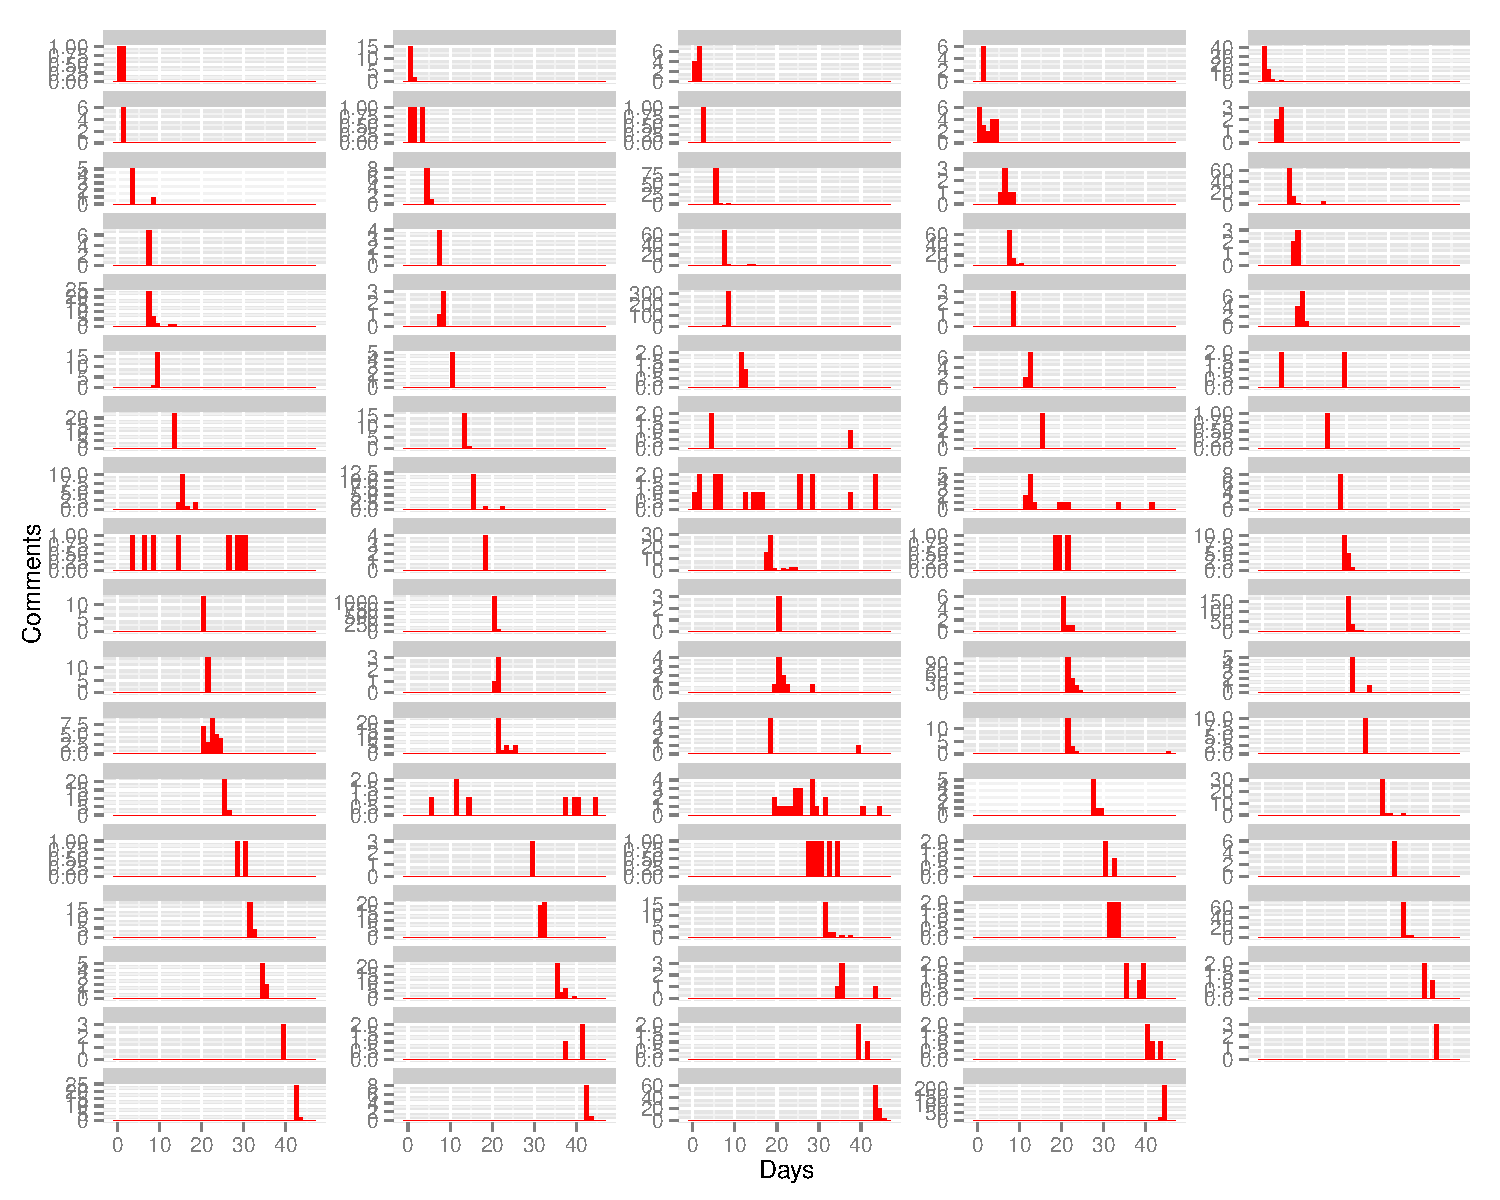
\includegraphics[width=9.5cm]{./imgs/DT_timebythread.pdf}
  \end{center}
\end{frame}

\begin{frame}\frametitle{Topics activity}
  \begin{center}
    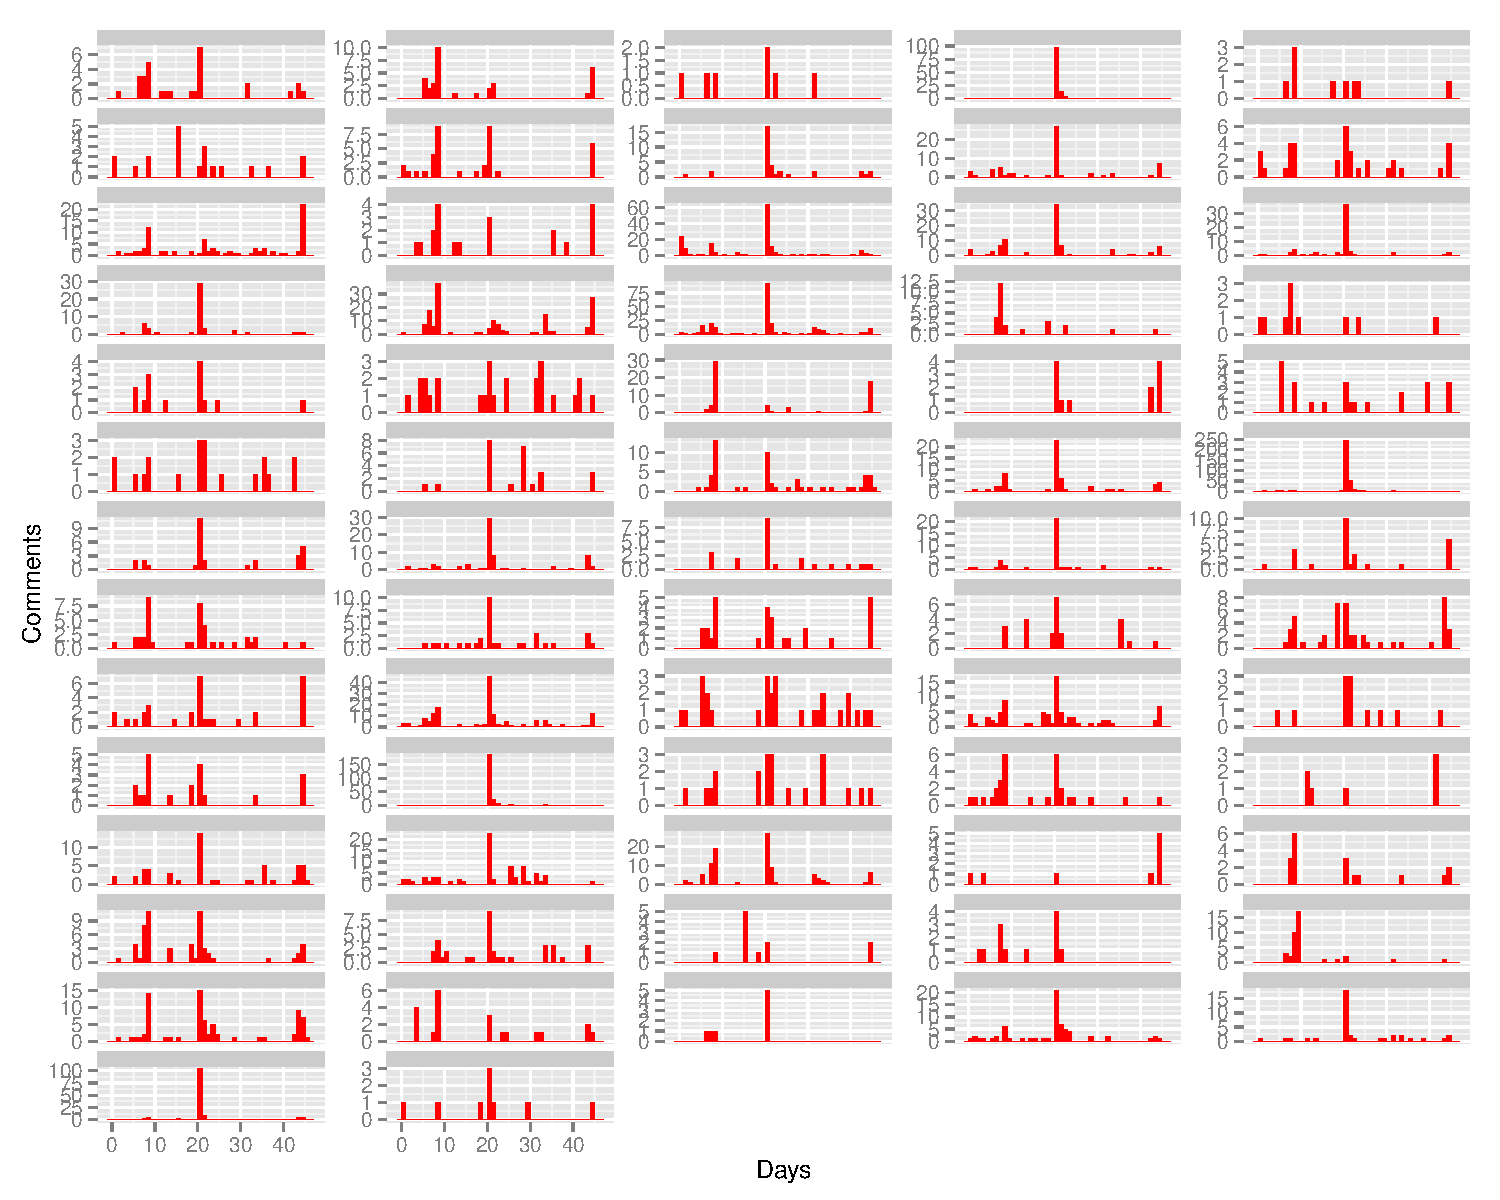
\includegraphics[width=9.5cm]{./imgs/DT_timebycluster.pdf}
  \end{center}
\end{frame}

\begin{frame}\frametitle{Topics $\times$ Threads}
  \begin{center}
    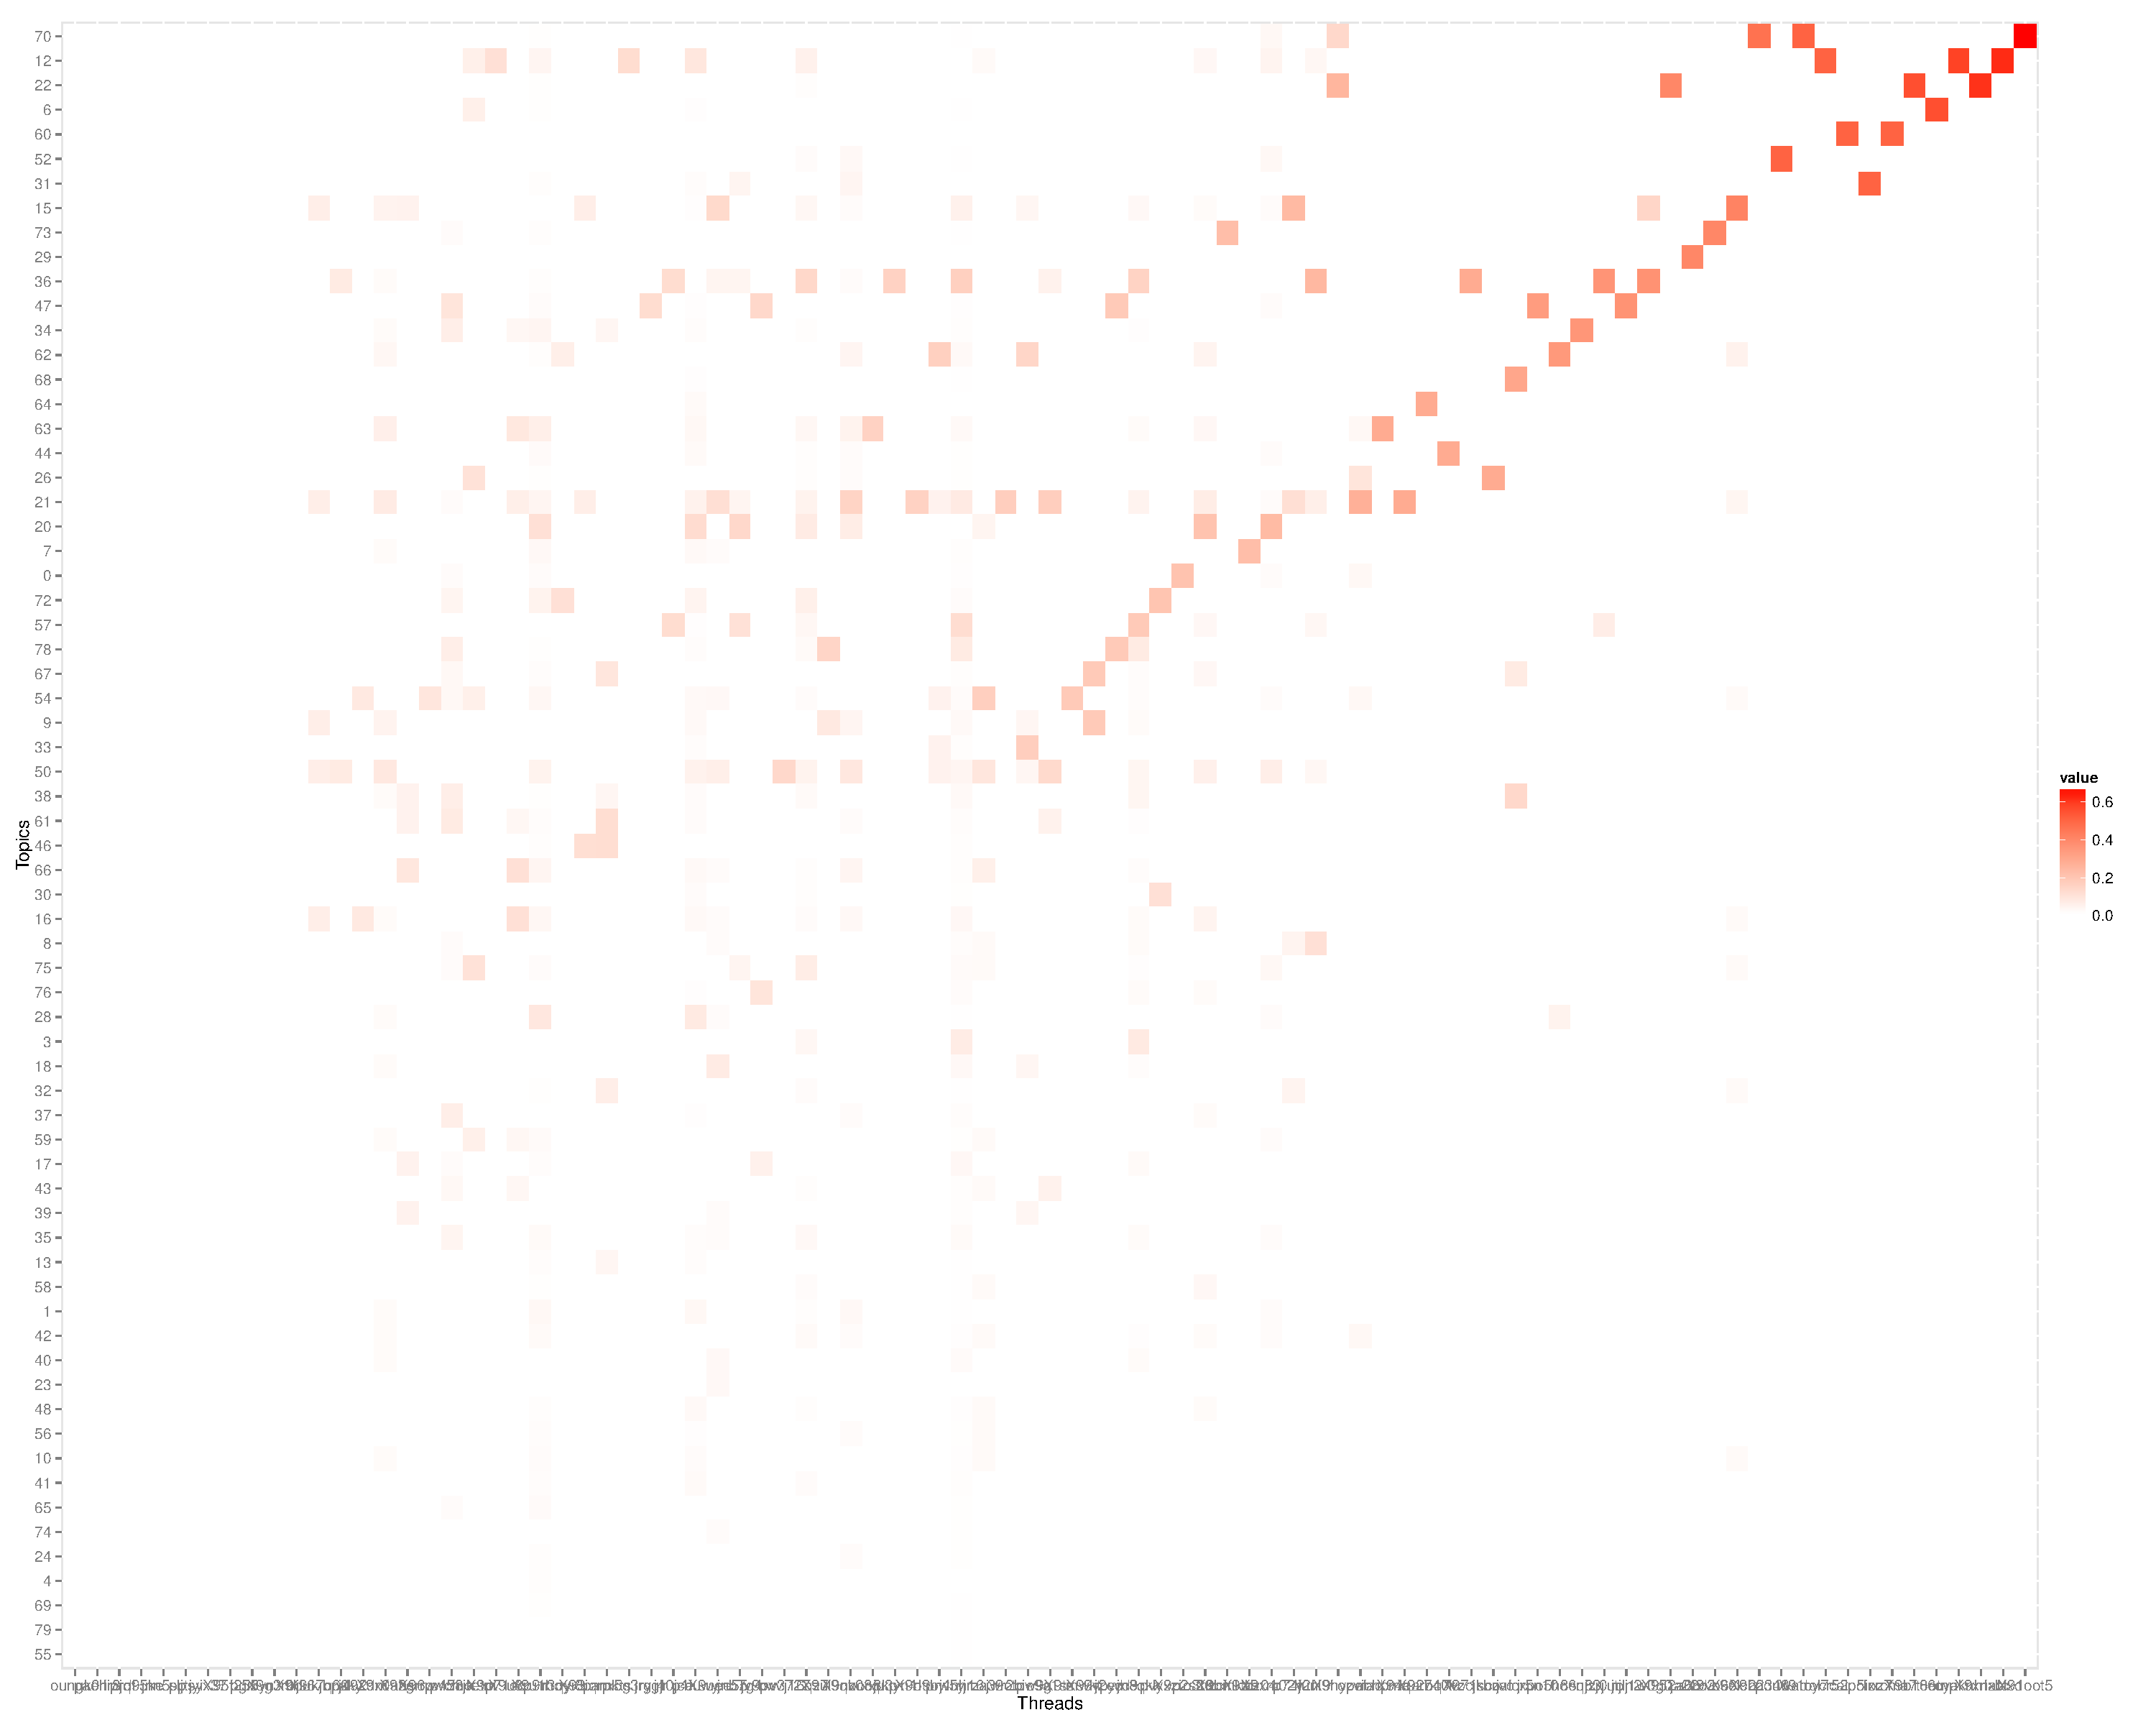
\includegraphics[width=9.5cm]{./imgs/DT_gg_heat.pdf}
  \end{center}
\end{frame}

\begin{frame}\frametitle{When we talk about texting and driving, we talk about \ldots}
\begin{center}
{\Large 
\begin{enumerate}
\item Topic 12: poor graphic design
\item Topic 50: fake ids and fake drivers licenses
\item Topic 58: health/accident insurance
\item Topic 62: drunk drivers
\item Topic 64: buses and bus drivers
\item Topic 67: bikes, bike lanes
\item Topic 68: trucks and truck drivers
\end{enumerate}
}
\end{center}
\end{frame}


%%%%%%%%
\section{Synthesis}
{
\usebackgroundtemplate{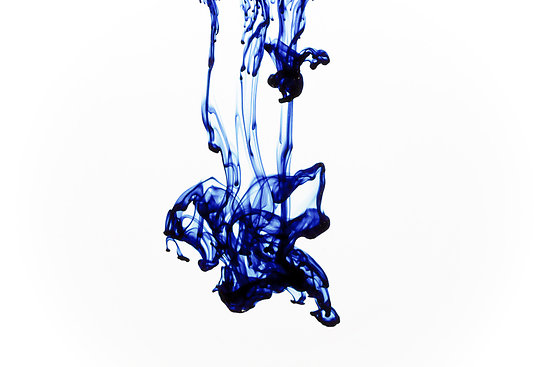
\includegraphics[width=7cm]{./imgs/ink.jpg}}
\begin{frame}
\textcolor{black} {
\hfill \Huge \insertsection}
\end{frame}
}

\begin{frame}\frametitle{Hamas vs. Israel in Gaza 2012}
  \begin{center}
    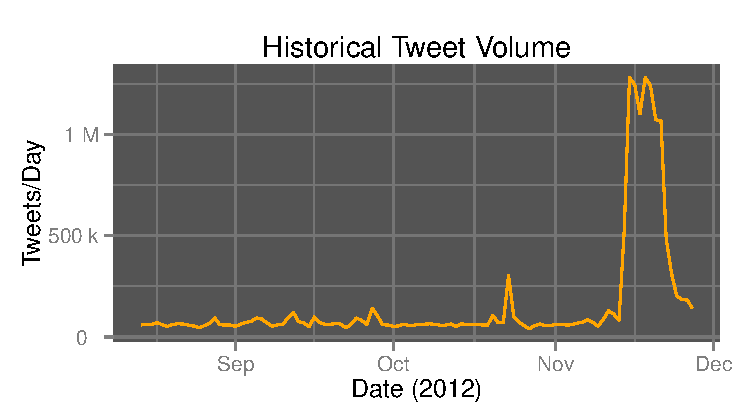
\includegraphics[width=10.5cm]{./imgs/HI_minimal-all-daily.pdf}
  \end{center}
\end{frame}

\begin{frame}\frametitle{What's that leading spike?}
  \begin{center}
    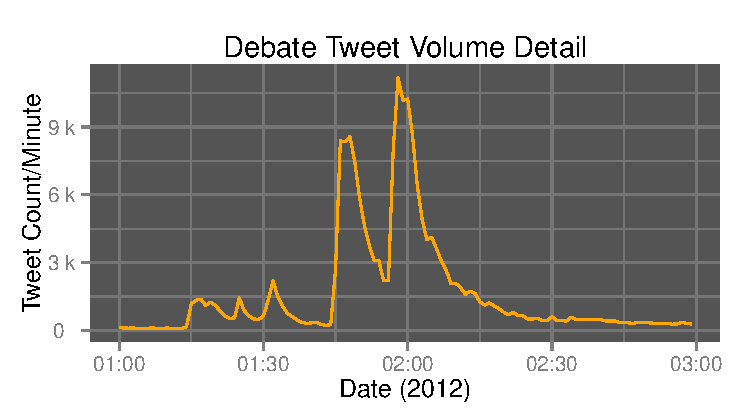
\includegraphics[width=10.5cm]{./imgs/HI_minimal-leadup-pres-debate.pdf}
  \end{center}
\end{frame}

\begin{frame}
  \begin{center}
    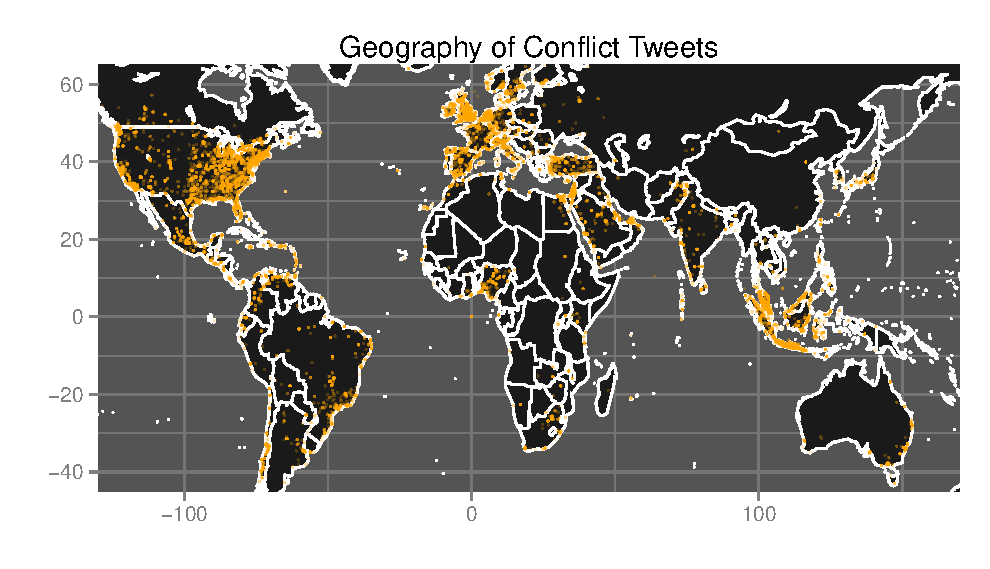
\includegraphics[width=11cm]{./imgs/HI_minimal-target-geo.pdf}
  \end{center}
\end{frame}

\begin{frame}\frametitle{Key accounts use of media}
  \begin{center}
    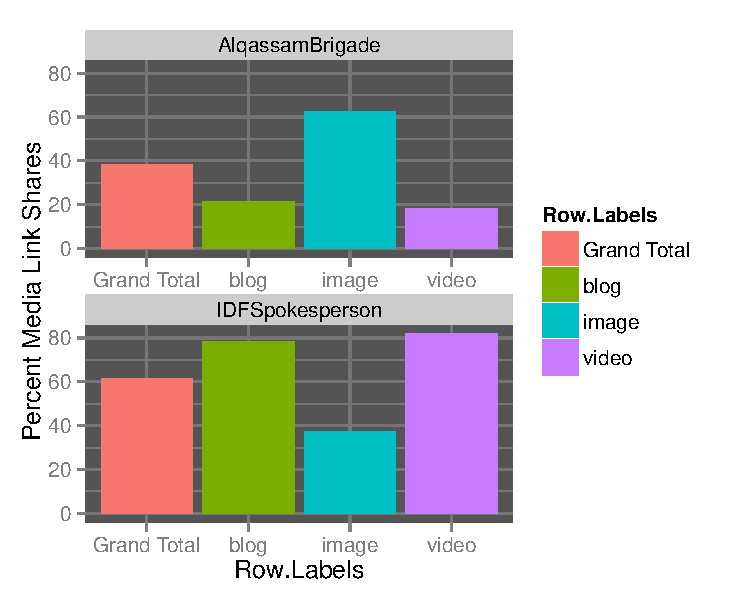
\includegraphics[width=9cm]{./imgs/HI_minimal-media.pdf}
  \end{center}
\end{frame}

\begin{frame}\frametitle{Conflict grows followers}
  \begin{center}
    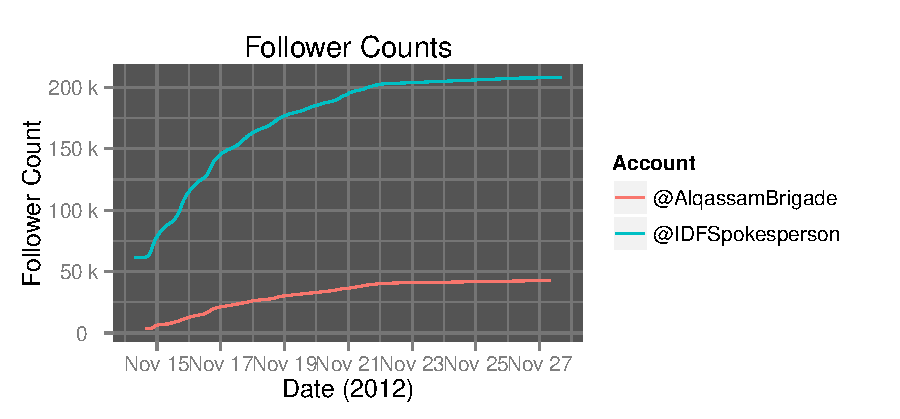
\includegraphics[width=10.5cm]{./imgs/HI_minimal-followers.pdf}
  \end{center}
\end{frame}


\begin{frame}\frametitle{Engagement with key accounts}
  \begin{center}
    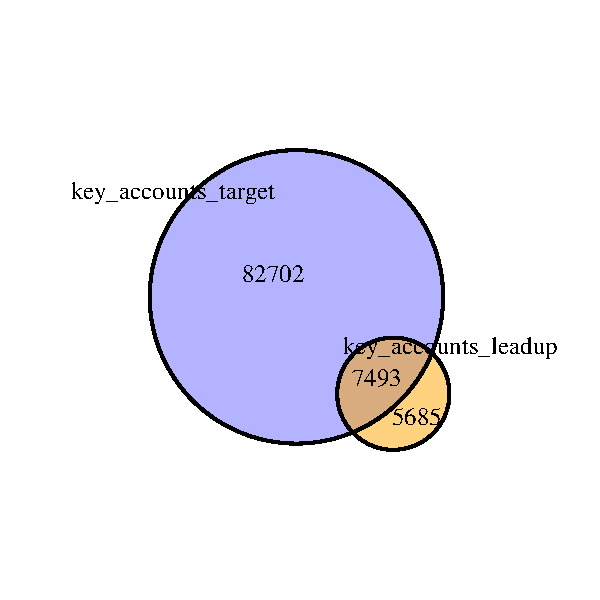
\includegraphics[width=8.5cm]{./imgs/HI_minimal-venns6.pdf}
  \end{center}
\end{frame}

\begin{frame}\frametitle{Crossover engagement}
  \begin{center}
    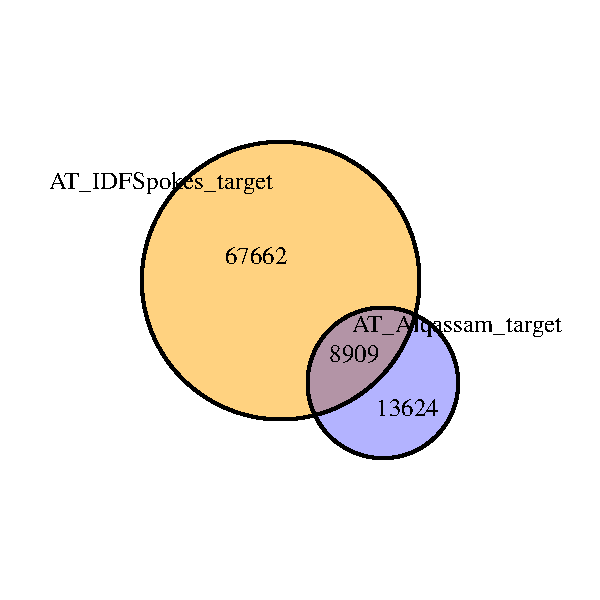
\includegraphics[width=8.5cm]{./imgs/HI_minimal-venns8.pdf}
  \end{center}
\end{frame}

%%%%%%%%
\section{Mixing it up}
{
\usebackgroundtemplate{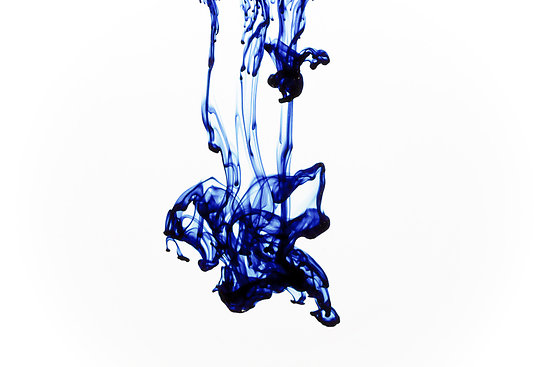
\includegraphics[width=7.5cm]{./imgs/ink.jpg}}
\begin{frame}
\textcolor{black} {
\Huge \hfill \insertsection}
\end{frame}
}

\begin{frame}
  \begin{center}
    \includegraphics[width=10cm]{./imgs/slide05.jpg}
  \end{center}
\end{frame}

\begin{frame}
  \begin{center}
    \includegraphics[width=10cm]{./imgs/slide06.jpg}
  \end{center}
\end{frame}

\begin{frame}
  \begin{center}
    \includegraphics[width=10cm]{./imgs/slide07.jpg}
  \end{center}
\end{frame}

\begin{frame}
  \begin{center}\frametitle{The Social Cocktail}
    \includegraphics[width=10cm]{./imgs/slide15.jpg}
  \end{center}
\end{frame}

% the end

\begin{frame}
  \begin{center}
    {\Large Thank you!}  \\ [20pt]
    
\includegraphics[width=3cm]{./imgs/logo.png} \\ [15pt]
    \begin{itemize}
    \item Presentation at: \url{http://github.com/DrSkippy27/Approach-to-Leveraging-Social-Data_2013}
    \end{itemize}
  \end{center}
\end{frame}

\end{document}
